\documentclass[conference,10pt,letterpaper]{IEEEtran}
\usepackage[T1]{fontenc}
\usepackage[utf8]{inputenc}
\usepackage{graphicx,booktabs,array,tabularx,url}
\usepackage[hidelinks]{hyperref}
\urlstyle{same}
\renewcommand{\ttdefault}{lmtt}
\graphicspath{{figures/}}
\hypersetup{pdftitle={Operating an Agent-Driven Dataset Factory: Discovery, Construction, and Public Release},pdfauthor={Eduardo Arino de la Rubia and Szilard Pafka}}
\title{Operating an Agent-Driven Dataset Factory:\\Discovery, Construction, and Public Release}
\author{\IEEEauthorblockN{Eduardo Ari\~no de la Rubia}\IEEEauthorblockA{Central European University\\\texttt{rubiae@ceu.edu}}\and\IEEEauthorblockN{Szilard Pafka}\IEEEauthorblockA{Epoch\\\texttt{szilard@epoch.com}}}
\begin{document}
\bstctlcite{IEEEexample:BSTcontrol}
\maketitle

\begin{abstract}
Turning public data into prediction datasets requires connecting source discovery, task definition, construction, and distribution. We deployed Dataset Factory to perform these steps continuously under a standing release policy. Bounded language-model tasks interpret sources, write construction code, and review task meaning; deterministic software manages state, workers, retries, and publication. Over 81.53 hours, the factory published 14 datasets at an estimated recurring operating expenditure of about \$2.74 per publication. The accounting includes failed attempts, inference, workers, and hosting. Separate agents completed prediction experiments on all twelve evaluated releases. Source review nevertheless identified a task whose construction filters contradicted its population declaration. The original reviewer accepted later-record exclusions without reconciling them with the published selection rule. This experience documents an operating source-to-release workflow and shows why successful execution and consumer use need separate checks of task meaning.
\end{abstract}
\begin{IEEEkeywords}agentic engineering, dataset construction, deployment experience, operating cost, semantic review\end{IEEEkeywords}

\section{Introduction}
Dataset Factory connected public-source discovery to fourteen published prediction datasets in an 81.53-hour deployment window. Separate agents completed modeling experiments on twelve of them. The same production process also accepted a task with a contradiction between its stated population and its construction filters. Together, these outcomes show what an automated workflow delivered and where its acceptance process fell short.

We built the factory for a small research group that needs unfamiliar, real-world prediction tasks. Public records require interpretation, filtering, labels, splits, and reproducible packaging before another researcher can use them. Analyst interviews and curation records document this work in discovery, transformation, and quality checks~\cite{kandel,lafia}. Automating a single step still leaves the problem of connecting the steps across sources.

This experience report contributes a concrete division of work between models and deterministic software, an operating record that includes repeated attempts and recurring expenditure, and an acceptance-failure analysis grounded in the original review inputs and response. We describe the system, report production and consumer use, and derive engineering lessons from the observed failures.

\section{System and Work Allocation}
\subsection{Discovery and construction}
Each release supplies a binary prediction task, training/validation/holdout splits, a predictor contract, construction code, a baseline, and source and license evidence. Matching versioned artifacts are published on GitHub and Hugging Face. The factory's code is public.\footnote{\url{https://github.com/earino/dataset-factory}}

Models interpret sources and generate code. The controller owns persistent state, resource limits, and external operations, so failed attempts can resume from recorded state.

A scheduled controller advances durable SQLite state through discovery, construction, evaluation, and publication (Fig.~\ref{fig:workflow}). It keeps up to two candidate slots pending. Each starts with a broad domain focus and the titles of previously selected tasks. The focus alternates infrastructure and environmental operations with institutions, commerce, transport, and public services.

The discovery model uses web search and extraction to inspect publisher downloads, field definitions, and redistribution terms. It returns a structured proposal with source evidence, the target, population, prediction time, available features, and fixed chronological splits, or defers the source with a reason. Code checks the required fields and rejects duplicate task identifiers. The model chooses the source and task; the controller decides whether the returned record can advance.

Construction is a separate model task without tools. It receives the source proposal and a descriptor schema, then returns Python code and task metadata. The builder writes the three splits and source checks. A temporary worker executes it, checks the full artifacts, and runs a fixed baseline. Checks cover file/schema compatibility, labels, splits, task-specific leakage checks, source evidence, and reproducibility records. Current-vintage retrospective tasks are permitted with declared assumptions; historical forecasting requires evidence of past input availability.

\begin{figure*}[t]
\centering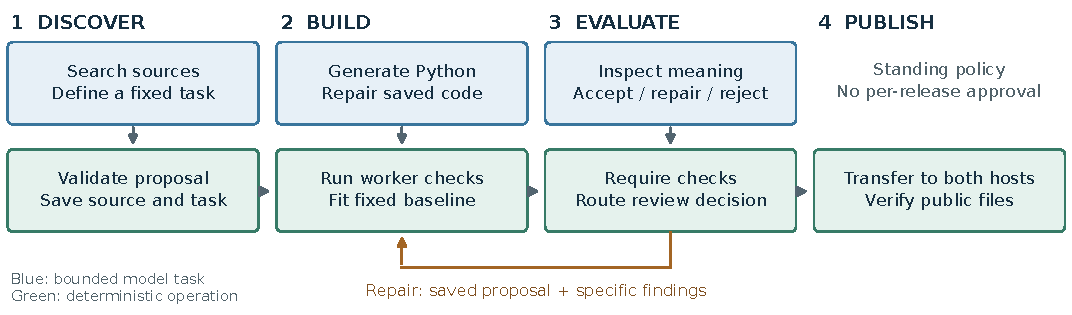
\includegraphics[width=\textwidth]{workflow.pdf}
\caption{Source-to-release workflow. Blue dashed boxes are model tasks; green solid boxes are code operations. Execution and semantic repairs return to builder generation.}
\label{fig:workflow}
\end{figure*}

\subsection{Review and bounded repair}
The semantic reviewer receives the source/task description, complete builder, construction notes, evaluation contract, and compact source, license, qualification, and baseline reports. It can consult publisher documentation and returns accept, repair, or reject with specific findings. Mechanical checks cannot be waived by that response. The review packet contains selected descriptor fields rather than the complete published descriptor, a distinction that matters in the failure examined in Section~\ref{sec:validity}.

Repairs receive saved proposals and bounded execution diagnostics or unresolved semantic findings. Unchanged proposal fields are reused. Access or terms failures can invoke web research for the same source; malformed responses can be repaired without repeating discovery. A rebuilt artifact must pass the worker checks and review again. The controller permits up to four semantic repair returns to construction before deferring further repair. Model-task and worker failures have separate five-failure limits per stage. Waiting for an existing worker is handled through recorded state.

Bounded model sessions run in Hermes Agent\footnote{\url{https://github.com/NousResearch/hermes-agent}}, using DeepSeek V4.1 Flash through Nous and Ollama Cloud. Research and review were capped at twelve tool-calling cycles, each comprising a model response and execution of its requested web tools. All tasks had a ten-minute timeout. Construction returns code for worker execution; it cannot run that code during generation. Models cannot directly launch workers, change coordinator state, or publish releases.

\subsection{Publication and autonomy}
One coordinator launches workers, preserves operation identities, and reconciles results; independent cleanup removes expired workers. A manifest binds accepted files to checksums. Workers retain source hashes and terms evidence; releases preserve upstream rights and attribution. Deterministic publication transfers the same files to both platforms and verifies anonymous access. Saved attempts and frozen releases preserve the evidence needed to resume work or inspect an earlier result.

A standing policy permits publication after artifact, semantic, and distribution checks, without per-dataset human approval. During the observation window, service administration changed the inference route and repaired worker-budget accounting. The inspected records show no manual changes to source selection, dataset construction, labels, or acceptance decisions.

\begin{table*}[t]
\caption{Publications in verification order: principal review findings and disclosure in pinned release documents.}
\label{tab:releases}
\centering\small
\renewcommand{\arraystretch}{1.17}
\setlength{\tabcolsep}{4pt}
\begin{tabular}{@{}>{\raggedright\arraybackslash}p{.25\textwidth}>{\raggedright\arraybackslash}p{.48\textwidth}>{\raggedright\arraybackslash}p{.235\textwidth}@{}}
\toprule
Task (domain) & Principal review finding & Release disclosure\\\midrule
\csname @@input\endcsname generated/release-rows.tex
\bottomrule
\end{tabular}
\end{table*}

\section{Observation and Evaluation Method}
\subsection{Production and expenditure}
Observation began with enrollment of new publications on 12 November 2026 at 21:28 UTC and ended on 16 November at 07:00 UTC, spanning 81.53 hours. Seven already-published pilot releases were excluded. A read-only export retains candidates, stage attempts, worker and inference usage, and publication identities. A candidate initially denotes a search slot. Milestones count distinct candidates; attempts count repeated stage work, including waiting or reconciliation rather than only distinct defects.

Recurring expenditure is estimated from recorded token categories, dated provider tariffs, worker lifetimes, and allocated hosting. Workers used Hetzner CPX32 servers with four allocated CPUs, a 30-minute task timeout, and a 60-minute lifetime limit. Inference pricing accounts for peak/off-peak timing; an all-peak calculation provides sensitivity. Earlier Nous-routed tokens are valued at direct DeepSeek rates. Workers use whole billed hours, and hosting is allocated from a \$20 monthly plan. These are resource-based estimates, not reconciled invoices.

Accounting includes unsuccessful production work and whole recorded session/worker lifetimes crossing the opening boundary, with worker exposure capped at close. It excludes development, human labor, upstream data collection, unmetered services, and the separate consumer evaluation. Expenditure divided by publications verified within the window is an operating ratio, not a lifetime construction cost.

\subsection{Consumer use and source review}
The consumer cohort comprises the first twelve new releases in publication-verification order, with their first accepted versions pinned. Separate Fable 5.2 agents under the same operator could modify XGBoost~\cite{xgboost} features, preprocessing, and parameters using training and labeled validation data within the predictor contract. Each release received three attempts of 85 minutes. Selected models were frozen before held-out scoring, which supplied one row at a time. Holdout access during research was procedurally prohibited. Provider failures and one premature stop were retried with unchanged release pins and budgets; their original records remain available.

We define \emph{usable} as supporting a completed prediction experiment under the predictor contract, ending in held-out scoring of a frozen model. This definition does not establish task validity.

For predictive performance, we compare consumers with an untuned XGBoost reference using 100 trees, depth 6, learning rate 0.1, and native categorical handling. A random-search control~\cite{randomsearch} tunes tree and sampling parameters on the same permitted inputs. Each control targets its paired consumer's fitting CPU from successful primary validation trials, subject to a wall-time cap and final-trial overshoot; inference, backtests, and other diagnostics are excluded. Consumers and controls select models by validation area under the ROC curve (AUC); final scoring uses held-out data to separate selection from evaluation~\cite{cawley}. Repeated-run studies motivate reporting variation~\cite{identical-runs}. We plot median paired AUC differences and ranges across three runs. Ranges describe observed run variation, not sampling uncertainty.

Separate bounded Fable reviews examined the pinned task descriptions, construction code, and permitted public data before scoring. They checked target meaning, timing, selection, splits, and label-derived history. The reviews shared instructions, but access to publisher documentation varied; raw source snapshots and holdout rows were outside their scope. Table~\ref{tab:releases} reports principal findings, distinguishing observed contradictions, unresolved concerns, and conditions of use. We compared each listed finding with the pinned release README and construction descriptor; \emph{not found} refers to these documents. Explicit isolated-row access counts as a stated restriction, even without an explanation of cross-row exposure. The final two production releases were outside both the consumer and separate-review cohort.

\begin{figure}[t]
\centering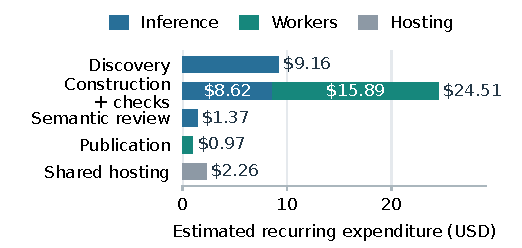
\includegraphics[width=\columnwidth]{stage-costs.pdf}
\caption{Estimated expenditure by stage at midpoint inference tariffs; construction includes checks and baseline fitting.}
\label{fig:costs}
\end{figure}

\begin{figure*}[t]
\centering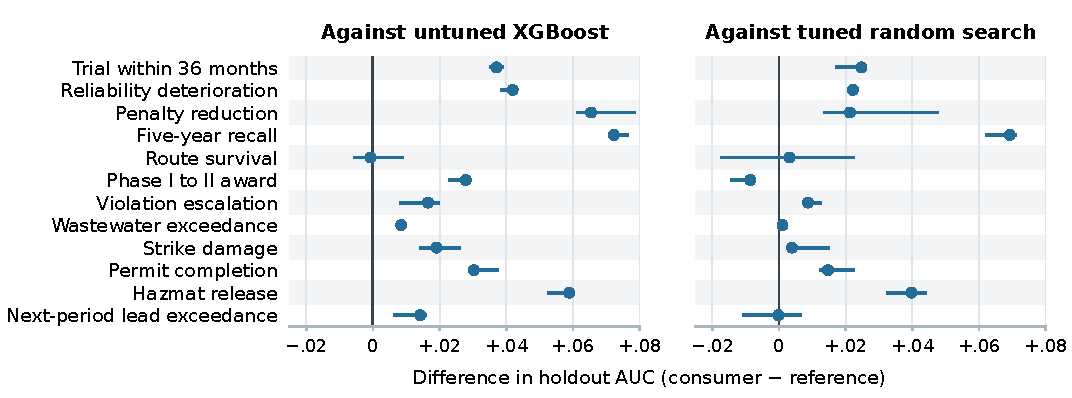
\includegraphics[width=\textwidth]{consumer-results.pdf}
\caption{Consumer AUC minus each reference. Points show median paired differences; bars span three runs. Positive values favor consumers.}
\label{fig:consumer}
\end{figure*}

\section{Deployment Results}
\subsection{Operation and recurring expenditure}
Fourteen releases were published. Fifty-four candidates completed discovery, eighteen a build, and fourteen acceptance and publication during the window. These are milestones in continuing operation. The record contains 540 stage attempts, including 101 discovery retries, 260 build retries, and 21 semantic repair outcomes across the factory. Among successful candidates, admission-to-publication time ranged from 40 to 231 minutes, with a median of 109.

The first publication illustrates the repair loop. For \emph{Trial within 36 months}, discovery completed at 00:57 UTC on 13 November. A descriptor failure and a failed worker build preceded the first qualified artifact. Semantic review then requested two repairs. The retained second review confirms that numeric coercion of court-district codes had been corrected to preserve letter-suffixed codes. The fifth build passed, the third review accepted, and both public destinations were verified at 02:30 UTC. These ten stage attempts include successful construction followed by further semantic repair.

A resource-accounting failure interrupted construction: worker reservations continued to consume the allowance after the workers had been deleted. A repair reconciled reservations with completed worker lifetimes and restored construction. The saved candidate state allowed work to continue.

Estimated recurring expenditure was \$38.23--\$38.33: \$19.10--\$19.21 for inference, \$16.86 for workers, and \$2.26 for hosting. The operating ratio was \$2.73--\$2.74 per publication. All-peak inference pricing raises it to \$3.92. Figure~\ref{fig:costs} attributes expenditure to recorded stages.

\subsection{Consumer use and predictive performance}
All twelve evaluated releases supported completed prediction experiments through held-out scoring. Consumer median AUC ranged from 0.601 to 0.913. Figure~\ref{fig:consumer} shows differences from both references. All three consumers scored above the untuned reference on eleven tasks; results for \emph{Route survival} were mixed. Median gains on those eleven tasks ranged from 0.008 to 0.072 AUC. All three paired point comparisons favored consumers on nine tasks, were mixed on \emph{Route survival} and \emph{Next-period lead exceedance}, and favored random search on \emph{Phase I to II award}. These comparisons concern the published splits and predictor contracts; the selection and timing findings in Table~\ref{tab:releases} remain material to their use.

Five of the six listed conditions of use were stated in the releases, including isolated-row access for both history-feature tasks. Carrier-code exits were disclosed, but apparent entries were not. Of the eight listed concerns, one was stated, three were partly stated, and four were not found in the inspected documents (Table~\ref{tab:releases}).

\subsection{A population contradiction survived acceptance}\label{sec:validity}
The \emph{Phase I to II award} task uses SBIR records to predict whether a firm's first Phase I award is followed by a Phase II award from the same agency within the next four fiscal years. Its published selection declaration says that outcome fields do not select rows. The builder nevertheless excludes firms with unknown award phases in the outcome window and firms with ambiguous phase or agency records. The release's limitations disclose some of these exclusions, contradicting its selection rule. Their effect on scores is unmeasured.

The original semantic reviewer received the complete builder, population description, passing check reports, and instructions to compare code with population rules. It did not receive the full published selection declaration. It explicitly accepted the later-record exclusions as label handling, concluded that the population matched the rule, and requested no repair. A separate pre-scoring review identified the contradiction from the published code and declaration. Inspection of the retained acceptance packet and response established this sequence. The record does not establish whether supplying the missing declaration would have changed acceptance.

A different condition appears in \emph{Wastewater exceedance}. A prior-year outcome is a legitimate input when available, but future rows can expose earlier labels through that feature. Our scorer supplies one row at a time; no leakage or consumer misconduct was observed in this scoring. Unrestricted batch use was not established safe.

\section{Engineering Lessons}
\textbf{Retain attempt and resource state} to expose repeated work and resume production after failures such as the worker-reservation error.

\textbf{Budget for execution as well as inference.} Construction, worker checks, and baseline fitting consumed 64\% of estimated expenditure (Fig.~\ref{fig:costs}); within that stage, worker charges exceeded inference charges.

\textbf{Review the claims that will be published.} For \emph{Phase I to II award}, checking the builder and a partial descriptor did not reconcile the selection declaration with its filters. We propose supplying the complete population/selection contract and requiring each inclusion rule to match it. This response has not been tested as a remedy.

\textbf{Specify the scoring interface.} The history feature in \emph{Wastewater exceedance} shows why accessible rows and outcomes belong in the task contract. Successful execution and legitimate per-row features do not establish safe use under every interface.

\section{Related Work}
AutoData~\cite{autodata-web} and DatasetResearch~\cite{datasetresearch} address web collection and dataset discovery. MLE-Smith~\cite{qiang2026mlesmith} constructs ML tasks from supplied datasets; AutoSDT~\cite{autosdt} searches repositories and adapts scientific programs into tasks. Their reported per-task costs use different output and accounting boundaries, so they cannot support an efficiency ranking with this deployment. Our contribution connects discovery, construction, public delivery, retained failures, and separate consumer use in one operating record.

MLAgentBench evaluates agents performing ML experiments~\cite{mlagentbench}. Here, consumer experiments characterize predictive performance on tasks produced by a separate factory. Studies of deployed agents emphasize reliability~\cite{production}, while AgentOps organizes the artifacts needed for lifecycle observability~\cite{agentops}. Jacobs and Wallach distinguish intended constructs from operational definitions~\cite{measurement}; the Agentic Benchmark Checklist separates task validity, outcome validity, and reporting~\cite{abc}. Datasheets connects provenance with intended use~\cite{datasheets}, and AutoDataBench examines generated task quality~\cite{autodatabench}.

\section{Limitations and Evidence}
This is one factory, one production-model family, and a short observation window. Public sources may have appeared in model training, and holdout isolation was procedural rather than technical. Source reviews were bounded and do not establish a defect rate across releases. Current-vintage records restrict historical forecasting claims: \emph{Trial within 36 months} inputs can postdate filing, \emph{Strike damage} and \emph{Hazmat release} use retrospective reports, and field-update timing remains unresolved for \emph{Permit completion}. Human policy, development, and responsibility remain outside the automated dataset decisions.

Release pins, operating records, transcripts, reviews, frozen models, and analysis code are retained in the study repository for public release at submission.\footnote{\url{https://github.com/earino/factory-prospective-study}}

\section{Conclusion}
Dataset Factory connected source discovery to public prediction datasets at about \$2.74 per publication in estimated recurring operating expenditure. Separate agents used twelve releases for prediction experiments, while source review exposed a population contradiction that automated acceptance missed. The experience supports engineering the complete workflow and checking task meaning separately from execution and consumer use.

\section*{AI Assistance}
AI systems assisted implementation, literature search, review briefs, source and transcript review, analysis, and drafting. Production and consumer models are identified above. The authors are responsible for the claims and final text.

\bibliographystyle{IEEEtran}
\bibliography{refs}
\end{document}
